\subsection{Opret Bruger}\label{sec:Opretbruger}
Dette afsnit indeholder en gennemgang af den grafisk brugergrænseflade, design og implementering af 'Opret Bruger' viewet i Rambøll Tilsyn.

\subsubsection{Design}
På Figur \ref{fig:OpretBrugerSekvens} ses sekvensdiagrammet for 'Opret bruger' viewet til Rambøll Tilsyn.
\begin{figure}[H] % (alternativt [H])
	\centering
	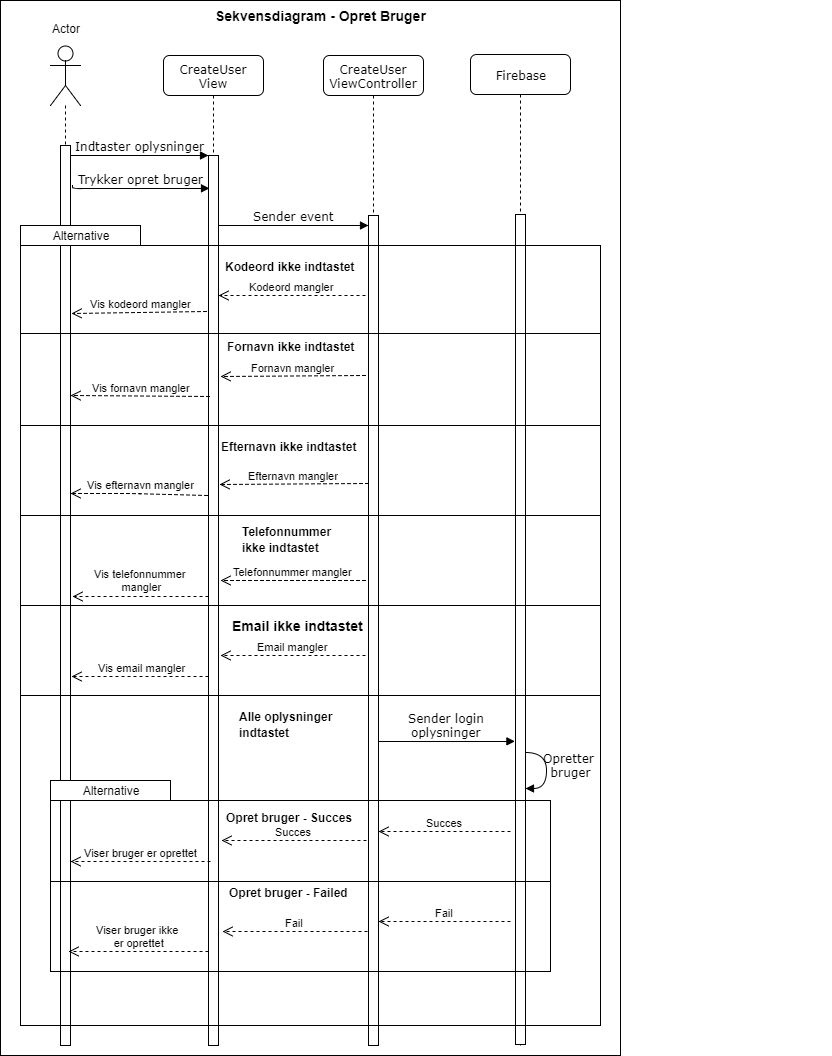
\includegraphics[height=20cm, width=15cm]{Design/Applikation/OpretBruger/OpretBrugerSekvensDiagram}
	\caption{Sekvensdiagram for 'Opret bruger' i Rambøll Tilsyn.}
	\label{fig:OpretBrugerSekvens}
\end{figure}

\subsubsection{Grafisk brugergrænseflade}
I OpretBrugerViewet er der lavet felter til alt den information, som skal tastes ind om en bruger. Se Figur \ref{fig:OpretBrugerView}
\begin{figure}[H] % (alternativt [H])
	\centering
	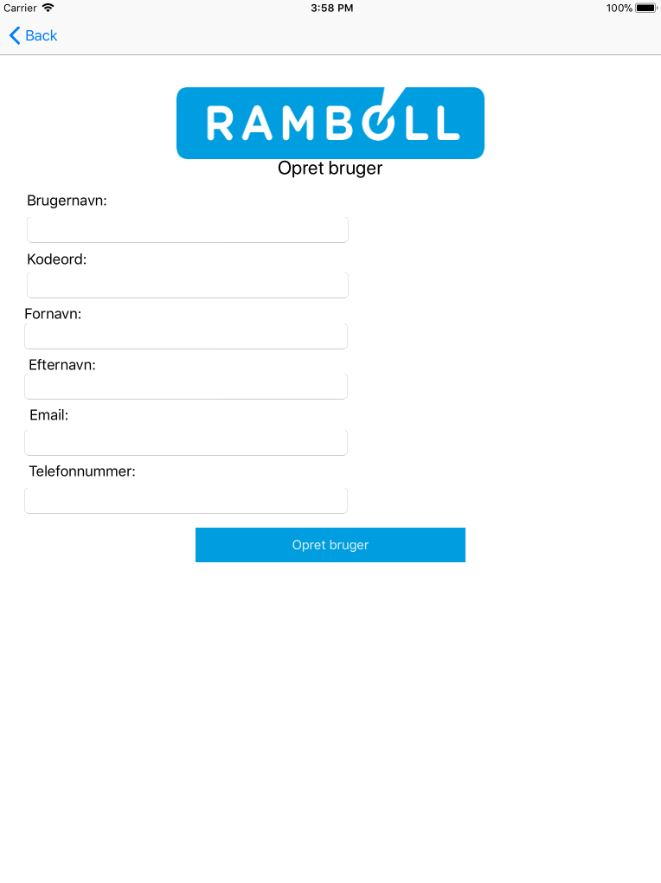
\includegraphics[height=12cm, width=10cm]{Design/Applikation/OpretBruger/OpretBrugerView}
	\caption{'Opret bruger' viewet, som det er implementeret i Rambøll Tilsyn.}
	\label{fig:OpretBrugerView}
\end{figure}

\subsubsection{Implementering}
Først valideres alle felterne og hvis inputs i alle felter bliver godkendte, oprettes brugeren der er indtastet i viewet. Når brugeren er oprettet korrekt, skrives informationen, der ikke er log ind specifikke ind i databasen. Dette er information som; fornavn og efternavn.


\clearpage